This section aims to expand upon the system definitions written in \autoref{user_requirements}, with the intention of establishing, and creating a better understanding of, a problem domain. This creates a set of tangible system requirements, that will help us define the basic classes and overall system structure.

%% cluster
To expand upon our system definition, a set of objects surrounding the system definition is set up to start working towards a solution, such an object could be a "tractor", "operator" or "agricultural equipment". These are all objects in their own, and are required to solve the process of tending a field, which is the first step in our system definition. Hence a list of objects that fulfills the system definition is listed below.

%% Complete List of Objects
\begin{itemize}[noitemsep]
    \item Tractor
    \item Combine
    \item Truck
    \item Plow
    \item Harrow
    \item Pesticide sprayer
    \item Manure spreader
    \item Fertilizer spreader
    \item Trailer
    \item Seeder
    \item Operator
    \item Seeds
    \item Manure
    \item Fertilizer
    \item Fuel
    \item Sensor
    \item GPS
    \item Field
\end{itemize}

These individual objects are setup in a \textbf{Cluster Diagram} to create an overview of which objects similar qualities, or interact with other objects, and thereby creating a baseline for classes that should represent a more streamlined diagram platform that we can work further on to create an end solution in later chapters. Such a \textbf{Cluster Diagram} is represented below in \autoref{fig:cluster_equipment}, and documented in appendix \autoref{appendix_cluster}. Here a representation of the overall object structure for \textbf{Agricultural Equipment} is shown, with all objects that are part of that object. Also, objects such as \textbf{GPS} and \textbf{Sensor}'s are part of the diagram, but are represented with a dotted line, to signify that these are not always part of the equipment.

\begin{figure}[ht]
    \centering
    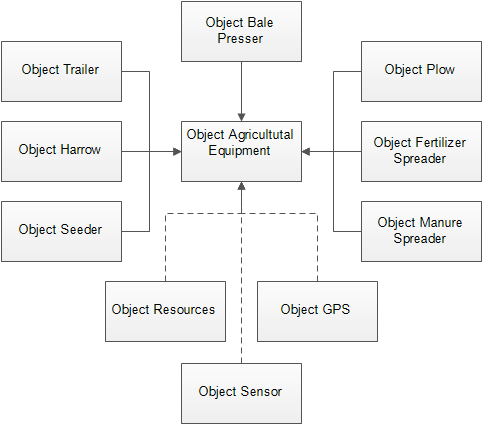
\includegraphics{images/cluster_diagram_agricultural_equipment}
    \caption{}
    \label{fig:cluster_equipment}
\end{figure}

%% structure


%% classes
%% - Definition
%% - Behavioral pattern